\section{Arquitectura y tecnologías de una aplicación web}
\label{sec:arquitectura_sistema}

En el mundo del software existen dos tipos de aplicaciones: las aplicaciones de escritorio y las aplicaciones web. Las aplicaciones de escritorio son aquellas que se instalan en un ordenador y se ejecutan de forma local, mientras que las aplicaciones web son aquellas que se ejecutan en un servidor y se acceden a través de un navegador web.

Desde los inicios del desarrollo de software, las aplicaciones de escritorio han sido la norma. Sin embargo, en los últimos años ha habido un cambio significativo hacia el desarrollo de aplicaciones web, pues el avance de las distintas tecnologías web y la conectividad a internet han mitigado considerablemente las desventajas que anteriormente presentaban \cite{evo_web}.

Las aplicaciones de escritorio no requieren de un servidor externo para funcionar, toda la lógica se encuentra en el ordenador del usuario y es este mismo quien lo ejecuta. Esto hace que la aplicación sea más rápida y eficiente, ya que no hay necesidad de enviar datos a través de internet. No obstante, esto también significa que el usuario debe instalar la aplicación en su ordenador y mantenerla actualizada, lo que puede ser un inconveniente \cite{web_vs_desktop}.

Por otro lado, las aplicaciones web sí que requieren de un servidor externo para funcionar. Esto significa que el usuario no necesita instalar nada en su ordenador, ya que la aplicación se ejecuta en el servidor y se accede a través de un navegador web. Este paradigma de desarrollo permite que la aplicación sea más accesible, pues se puede acceder a la aplicación desde cualquier dispositivo y lugar con conexión a internet. Además, como todo se encuentra en el servidor y no en el usuario, las actualizaciones son mucho más inmediatas. Sin embargo, esto también significa que la aplicación puede ser más lenta y menos eficiente debido a que la lógica y los datos no se encuentran en el ordenador del usuario, sino en el servidor \cite{web_vs_desktop}.

La mejor conectividad a internet y el avance de las tecnologías web han permitido que las aplicaciones web sean cada vez más rápidas y eficientes. Esto ha llevado a un aumento en la popularidad de las aplicaciones web, y muchas empresas están optando por desarrollar aplicaciones web en lugar de aplicaciones de escritorio.

Con todo esto, se ha formado lo que se conoce como arquitectura web, que hace referencia a la forma en que se organiza y estructura el software. Esto incluye la forma en que se comunican los diferentes componentes de la aplicación, así como la forma en que se almacenan y gestionan los datos. Todas las aplicaciones web están compuestas por tres componentes principales: el cliente, la lógica de negocio y la base de datos.

Estos tres componentes se dividen en dos bloques: el \textit{frontend} y el \textit{backend}. El \textit{frontend} es la parte de la aplicación que interactúa con el usuario, es decir, el cliente, mientras que el \textit{backend} es la parte de la aplicación que se encarga de gestionar los datos y la lógica de negocio. Ambos bloques se comunican entre sí a través de una API (Interfaz de Programación de Aplicaciones), que es un conjunto de reglas y protocolos que permiten que diferentes componentes de software se comuniquen entre sí. Todo esto se puede ver en la figura \ref{fig:arquitectura_web}.

\begin{figure}
    \centering
    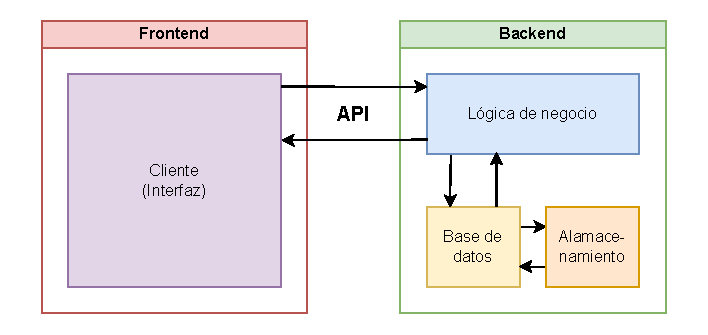
\includegraphics[width=0.8\textwidth]{figures/theoric_frame/arquitectura_web.pdf}
    \caption{Arquitectura de una aplicación web.}
    \label{fig:arquitectura_web}
\end{figure}

\subsection{\textit{Frontend}}
\label{mt:subsec:frontend}

El \textit{frontend} es la parte de la aplicación que interactúa con el usuario. Esto incluye la interfaz de usuario, que es la parte de la aplicación que el usuario ve y con la que interactúa, así como la lógica de presentación, que es la parte de la aplicación que se encarga de mostrar los datos al usuario. El \textit{frontend} se desarrolla principalmente utilizando HTML, CSS y JavaScript, tecnologías que se ejecutan de manera nativa en los navegadores.

El HTML (\textit{Hypertext Markup Language}) es el lenguaje de marcado utilizado para estructurar el contenido de una página web. El CSS (\textit{Cascading Style Sheets}) es el lenguaje utilizado para dar estilo a una página web, es decir, para definir cómo se verá el contenido estructurado por el HTML. Por último, JavaScript es un lenguaje de programación que se utiliza para añadir interactividad a una página web, es decir, para permitir que el usuario interactúe con la aplicación.

Con todo esto, el servidor envía todo este contenido al usuario de manera que su navegador lo pueda representar, en caso del HTML y el CSS, y ejecutar, en caso del JavaScript.

Desarrollar aplicaciones de manera nativa, es decir, utilizando HTML, CSS y JavaScript sin el apoyo de ninguna librería o herramienta adicional, puede ser complicado, tedioso y poco eficiente. Para facilitar esta tarea, existen distintos \textit{frameworks} que proporcionan un conjunto de herramientas y funcionalidades pensadas para abstraer la complejidad del desarrollo. De esta manera, los \textit{frameworks} cumplen principalmente dos propósitos:

\begin{itemize}
    \item \textbf{Ahorrar tiempo:} Los \textit{frameworks} permiten al desarrollador ahorrar tiempo ofreciendo funcionalidades predefinidas a problemas comunes o recurrentes. En el caso de una aplicación web, esto puede incluir la gestión de rutas, la gestión del estado de la aplicación, la gestión de formularios, entre otros \cite{framworks}.
    \item \textbf{Garantizar buenas prácticas de desarrollo:} Los \textit{frameworks} suelen seguir patrones de diseño y buenas prácticas de desarrollo que ayudan a los desarrolladores a escribir código limpio, mantenible y escalable. Adicionalmente ofrecen características de seguridad por defecto, de manera que el desarrollador no tiene que implementar sus propias medidas de seguridad que pueden resultar ser vulnerables. Un ejemplo es la autenticación de usuarios, donde el \textit{framework} se encarga de gestionar la creación y validación de los \textit{tokens} de acceso, así como la gestión de sesiones \cite{framworks}.
\end{itemize}

Algunos de los \textit{frameworks} más populares para el desarrollo de \textit{frontend} son React, Angular y Vue.js. En el caso de este proyecto, se ha optado por utilizar React, un \textit{framework} desarrollado por Facebook que en los últimos años se ha convertido en un estándar de la industria. React es un \textit{framework} basado en componentes, lo que significa que la interfaz de usuario se divide en unidades independientes y reutilizables, facilitando así la creación de aplicaciones más complejas y escalables.

React se desarrolla utilizando JavaScript, un lenguaje de programación de tipado dinámico, lo que significa que no requiere de declarar el tipo de las variables al momento de crearlas. Esta característica, si bien ofrece flexibilidad, puede provocar errores difíciles de detectar. Para solventarlo, existe TypeScript, un lenguaje que extiende JavaScript añadiendo tipado estático \cite{typescript}. Con TypeScript, el desarrollador puede especificar el tipo de las variables, permitiendo que los errores de tipado se detecten en tiempo de interpretación. Aunque los navegadores solo interpretan JavaScript, el código en TypeScript se transpila automáticamente a JavaScript. Por este motivo, en este proyecto se ha decidido utilizar TypeScript para mejorar la calidad y la robustez del código \cite{tipado}.

Finalmente, otro motivo relevante para la elección de React es su gran comunidad de desarrolladores, así como la amplia disponibilidad de librerías y herramientas que extienden sus funcionalidades básicas. La elección de React y el detalle de su funcionamiento se explican en profundidad en la sección \textcolor{red}{(Añadir sección parte desarrollo frontend)}.

\subsection{\textit{Backend}}
\label{subsec:backend}

El \textit{backend} es la parte de la aplicación que administra la funcionalidad general de la aplicación. Cuando el usuario interactúa con el \textit{frontend}, la interacción envía una solicitud al \textit{backend} para que la procese y devuelva una respuesta \cite{aws_frontend_backend}. De este modo, el \textit{backend} se encarga de gestionar la lógica de negocio, es decir, es la parte de la aplicación que se encarga de procesar los datos y realizar las operaciones necesarias para realizar las distintas funcionalidades de ésta. Adicionalmente contiene la base de datos, que es donde se almacenan todos los datos de la aplicación.

A diferencia del \textit{frontend}, el \textit{backend} no se ejecuta en el navegador del usuario, sino en un servidor. Esto significa que el \textit{backend} puede utilizar lenguajes de programación y tecnologías que no son compatibles con los navegadores, como Java, Python o Ruby. No obstante, un factor que si tiene en común con el \textit{frontend} es la existencia de \textit{frameworks}.

Para el desarrollo de este proyecto se ha decidido utilizar Django, un \textit{framework} escrito en Python. Django es un \textit{framework} un tanto especial, ya que permite desarrollar tanto el \textit{frontend} como el \textit{backend} de una aplicación web. Sin embargo, en este proyecto se ha optado por utilizar Django únicamente para el desarrollo del \textit{backend}, dejando el \textit{frontend} a cargo de React, pues se considera que es la mejor opción para el desarrollo de aplicaciones web modernas. En cuanto al aspecto más técnico, Django está basado en el modelo MVC (Modelo-Vista-Controlador), un patrón de diseño que separa la lógica en tres componentes principales: el modelo, que se encarga de gestionar los datos; la vista, que se encarga de mostrar los datos al usuario; y el controlador, que se encarga de gestionar la interacción entre el modelo y la vista \cite{mvc}.

El funcionamiento del modelo MVC se representa en la figura \ref{fig:mvc}. Para entender mejor este flujo, se puede tomar como ejemplo una acción concreta dentro del proyecto: acceder a la sección de productos de la aplicación. A continuación, se explica paso a paso lo que ocurre en ese proceso:

\begin{enumerate}
    \item \textbf{Solicitud del usuario} El usuario accede a la sección de productos desde el \textit{frontend}, ya sea a través de un menú o directamente introduciendo una URL. Esta acción genera una solicitud HTTP que se envía a un \textit{endpoint} del \textit{backend} (paso 1 en la figura).
    \item \textbf{Recepción por parte del controlador:} El \textit{endpoint} está vinculado a una función del controlador, que es el encargado de procesar la solicitud. En este caso, el controlador interpreta que se necesita acceder a los datos de los productos y actúa en consecuencia (paso 2).
    \item \textbf{Consulta al modelo:} El controlador solicita la información al modelo correspondiente, es decir, a los productos. El modelo representa la estructura de datos y contiene la lógica necesaria para interactuar con la base de datos de manera más sencilla y segura (paso 3).
    \item \textbf{Respuesta del modelo:} El modelo realiza la consulta a la base de datos y devuelve al controlador los datos solicitados, en este caso, la lista de productos (paso 4).
    \item \textbf{Selección de la vista:} Con los datos recibidos, el controlador selecciona la vista adecuada para estructurar la respuesta. Esta vista se encarga de preparar los datos en un formato que el \textit{frontend} pueda interpretar, normalmente JSON (\textit{JavaScript Object Notation}) (paso 5).
    \item \textbf{Respuesta al usuario:} La vista estructurada en formato JSON se devuelve al controlador, que finalmente la envía como respuesta al usuario. El \textit{frontend} recibe estos datos y se encarga de representarlos en la interfaz gráfica, mostrando al usuario la información solicitada: los productos (paso 6).
\end{enumerate}

\begin{figure}
    \centering
    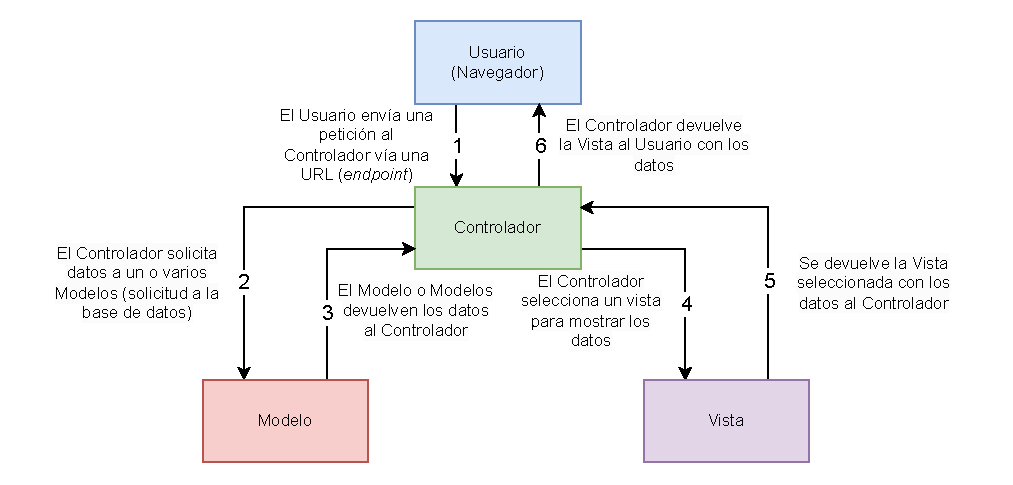
\includegraphics[width=0.8\textwidth]{figures/theoric_frame/mvc.pdf}
    \caption{Diagrama de flujo del patrón de diseño MVC.}
    \label{fig:mvc}
\end{figure}

Una mayor profundidad sobre el funcionamiento de los modelos y la base de datos se puede encontrar en la sección \ref{mt:subsec:base_datos} y sobre la comunicación entre el \textit{frontend} y el \textit{backend} en la sección \ref{mt:subsec:api}.

\subsection{Base de datos}
\label{mt:subsec:base_datos}

La base de datos es una colección de datos electrónicamente almacenados y organizados de manera que se puedan acceder, gestionar y actualizar fácilmente. En el caso de una aplicación web, la base de datos se utiliza para almacenar toda la información necesaria para el funcionamiento de ésta \cite{aws_database}.

Existen distintos tipos de bases de datos, pero las más comunes son las bases de datos relacionales y las bases de datos no relacionales. Las bases de datos relacionales almacenan los datos en tablas, donde cada fila representa un registro y cada columna representa un campo. Este tipo de base de datos es ideal para aplicaciones que requieren una estructura de datos rígida y bien definida. Por otro lado, las bases de datos no relacionales almacenan los datos en formatos más flexibles, como documentos o pares clave-valor. Este tipo de base de datos es ideal para aplicaciones que requieren una estructura de datos más flexible y escalable \cite{aws_database_rel}.

En este proyecto se ha optado por utilizar una base de datos relacional, pues la mayoría de los datos que se gestionan son estructurados y requieren una relación entre ellos. Así pues, se ha decidido usar PostgreSQL, un sistema de gestión de bases de datos relacional de código abierto que funciona de manera nativa con Django.

Con el tipo de base de datos definido, es fundamental comprender el funcionamiento básico de una base de datos relacional. Este tipo de base de datos organiza la información en tablas, cada una con un nombre específico. Las tablas están compuestas por un conjunto fijo de columnas, que representan los campos o atributos de los datos, y un conjunto variable de filas, donde cada una corresponde a un registro u objeto dentro de la tabla. Cada fila, es decir, cada registro, tiene un identificador único conocido como clave primaria, que permite distinguirlo de los demás registros de la tabla y relacionarlo con otras tablas a partir de claves foráneas. Las claves foráneas son columnas que establecen una relación entre dos o más tablas, permitiendo que los datos de una tabla se vinculen con los datos de otras. Esto es especialmente útil para representar relaciones entre diferentes entidades dentro de la base de datos, como por ejemplo, la relación entre un pedido, el cliente que lo ha realizado y sus productos asociados, tal como se muestra en la figura \ref{fig:rel_db}.

\begin{figure}
    \centering
    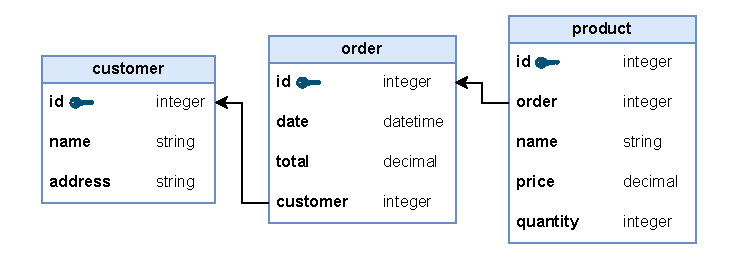
\includegraphics[width=0.8\textwidth]{figures/theoric_frame/rel_db.pdf}
    \caption{Tablas de ejemplo de una base de datos para guardar pedidos.}
    \label{fig:rel_db}
\end{figure}

Para crear, modificar, eliminar y consultar los datos de una base de datos relacional, se utiliza SQL (\textit{Structured Query Language}), un lenguaje de programación diseñado específicamente para gestionar bases de datos. SQL permite realizar operaciones como la creación de tablas, la inserción de datos, la actualización de registros y la consulta de información \cite{aws_sql}. No obstante, realizar consultas SQL directamente puede ser complicado y propenso a errores, especialmente en aplicaciones más complejas. \textcolor{red}{Explicar fallos seguridad, querys mal optimizadas...} Por este motivo, Django ofrece una capa de abstracción llamado sistema ORM (\textit{Object-Relational Mapping}), que permite interactuar con la base de datos utilizando objetos y clases de Python en lugar de escribir consultas SQL directamente. De esta manera, con ORM cada tabla de la base de datos es representada por lo que se llama un modelo, que es una clase de Python que define la estructura de la tabla y sus relaciones con otras tablas. Cada instancia de un modelo representa una fila en la tabla correspondiente, y los atributos de la clase representan las columnas de la tabla. Este enfoque se puede ver ejemplificado en la figura \ref{fig:orm_vs_sql}, donde se muestra una consulta SQL y su equivalente en ORM para obtener los campos \texttt{total} y \texttt{date} del registro que tiene \texttt{customer = 7} de la tabla \texttt{order}.

\begin{figure}[H]
    \centering
    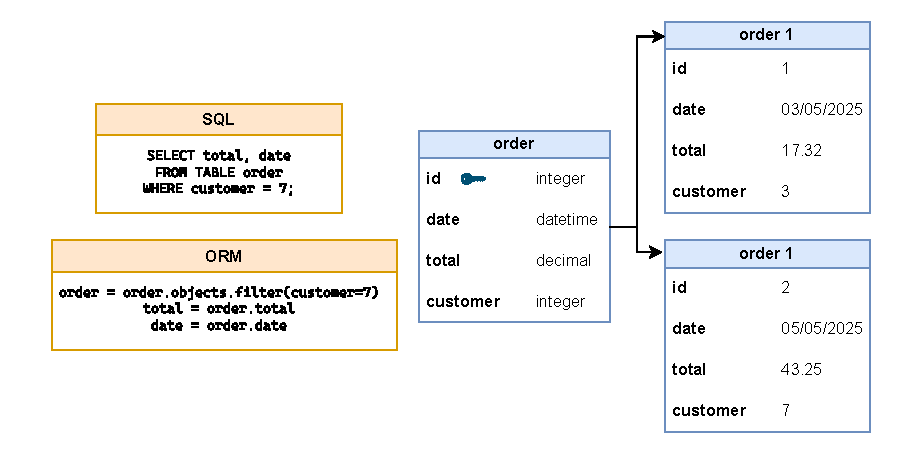
\includegraphics[width=0.8\textwidth]{figures/theoric_frame/orm_vs_sql.pdf}
    \caption{Ejemplo de consulta SQL y su equivalente en ORM para la obtención de dos campos de un registro de una tabla.}
    \label{fig:orm_vs_sql}
\end{figure}

\subsection{API}
\label{mt:subsec:api}

La API (\textit{Application Programming Interface}) es un conjunto de mecanismos que permiten la comunicación entre diferentes componentes de software mediante unas definiciones y unos protocolos. En el caso de una aplicación web, la API es la interfaz que permite al \textit{frontend} comunicarse con el \textit{backend} y viceversa. Esto significa que cuando el usuario interactúa con el \textit{frontend} se envían solicitudes a la API (al \textit{backend}), que las procesa y devuelve una respuesta. No obstante, las API no solo permiten la comunicación entre el \textit{frontend} y el \textit{backend}, sino que también permiten la comunicación entre diferentes aplicaciones. Un ejemplo que aplica a este proyecto es la comunicación entre el \textit{backend} de la aplicación y un \textit{marketplace}, donde se emplea una API. Para obtener un pedido de un \textit{marketplace}, el \textit{backend} debe enviar una solicitud a la API del \textit{marketplace} y recibe una respuesta con la información del pedido \cite{aws_api}.

La arquitectura de una API se entiende en términos de cliente y servidor, de manera que la aplicación que envía la solicitud se llama cliente y la aplicación que recibe y procesa la solicitud se llama servidor. En el ejemplo anterior, el \textit{backend} actua como cliente y el \textit{marketplace} actua como servidor.

Sin embargo, las API pueden ser de distintos tipos, dependiendo de cómo se estructuren y cómo se comuniquen. En el caso de este proyecto, se ha optado por utilizar una API REST (\textit{Representational State Transfer}), que son las más comunes en la actualidad. Una API REST es un tipo de API que utiliza el protocolo HTTP para la comunicación entre el cliente y el servidor, lo que significa que las solicitudes y respuestas se envían a través de HTTP, utilizando principalmente los siguientes métodos para realizar operaciones sobre los recursos:

\begin{itemize}
    \item \textbf{GET:} Se utiliza para obtener información de un recurso. Por ejemplo, si se quiere obtener la lista de productos de la aplicación, se enviaría una solicitud GET a la API con la URL correspondiente.
    \item \textbf{POST:} Se utiliza para crear un nuevo recurso. Por ejemplo, si se quiere crear un nuevo producto, se enviaría una solicitud POST a la API con la información del producto en el cuerpo de la solicitud.
    \item \textbf{PUT:} Se utiliza para actualizar un recurso existente. Por ejemplo, si se quiere actualizar la información de un producto, se enviaría una solicitud PUT a la API con la información actualizada en el cuerpo de la solicitud.
    \item \textbf{PATCH:} Se utiliza para actualizar parcialmente un recurso existente. Por ejemplo, si se quiere actualizar solo el precio de un producto, se enviaría una solicitud PATCH a la API con la información actualizada en el cuerpo de la solicitud.
    \item \textbf{DELETE:} Se utiliza para eliminar un recurso. Por ejemplo, si se quiere eliminar un producto, se enviaría una solicitud DELETE a la API con la URL del producto a eliminar.
\end{itemize}

Tal como se puede observar en los ejemplos de cada uno de los métodos, la API REST utiliza URLs para identificar los recursos. Cada recurso tiene una URL única que se utiliza para acceder a él. Por ejemplo, la URL para acceder a la lista de productos podría ser \texttt{https://api.ejemplo.com/products}, mientras que la URL para acceder a un producto específico podría ser \texttt{https://api.ejemplo.com/products/1}, donde el número 1 representa el identificador único del producto. Algunos métodos, como pueden ser el POST y el PATCH incluyen un \textit{body}, que es el cuerpo de la solicitud, donde se encuentran los datos que se envían en la petición.

Tanto el \textit{body} como la respuesta de la API acostumbran a estar en formato JSON, un formato basado en texto estructurado de manera que permite representar datos de manera sencilla y legible. En la figura \ref{fig:api_example} se puede ver un ejemplo de una petición a una API REST y la respuesta en formato JSON. En este caso, se está realizando una petición GET a la API para obtener el producto que tiene \texttt{id = 1}, y la respuesta es un objeto JSON que contiene la información de dicho producto.

\begin{figure}[H]
    \centering
    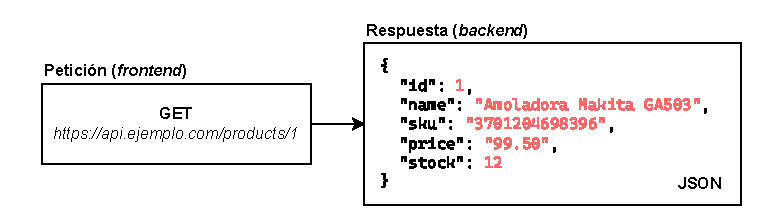
\includegraphics[width=0.8\textwidth]{figures/theoric_frame/api_example.pdf}
    \caption{Ejemplo de una petición a una API REST con la correspondiente respuesta en formato JSON.}
    \label{fig:api_example}
\end{figure}

Por último, es importante destacar los llamados \textit{query parameters}, que son parámetros que se pueden añadir a la URL para filtrar o modificar la respuesta de la API. Por ejemplo, si se quiere obtener solo los productos que tienen stock, se podría añadir un parámetro a la URL como \texttt{?stock=true}. Esto permite que la API devuelva solo los productos que cumplen con ese criterio, lo que puede ser útil para optimizar las consultas y reducir la cantidad de datos transferidos. De esta manera, para obtener los productos que están en oferta, la URL de la API podría ser \texttt{https://api.ejemplo.com/products?stock=true}. Esto puede verse en la figura \ref{fig:query_params_example}, donde se muestra un ejemplo de una respuesta a una petición sin y con \textit{query parameters}. En este caso, la primera respuesta devuelve todos los productos, mientras que la segunda respuesta devuelve solo los productos que tienen un stock superior a 0.

\begin{figure}[H]
    \centering
    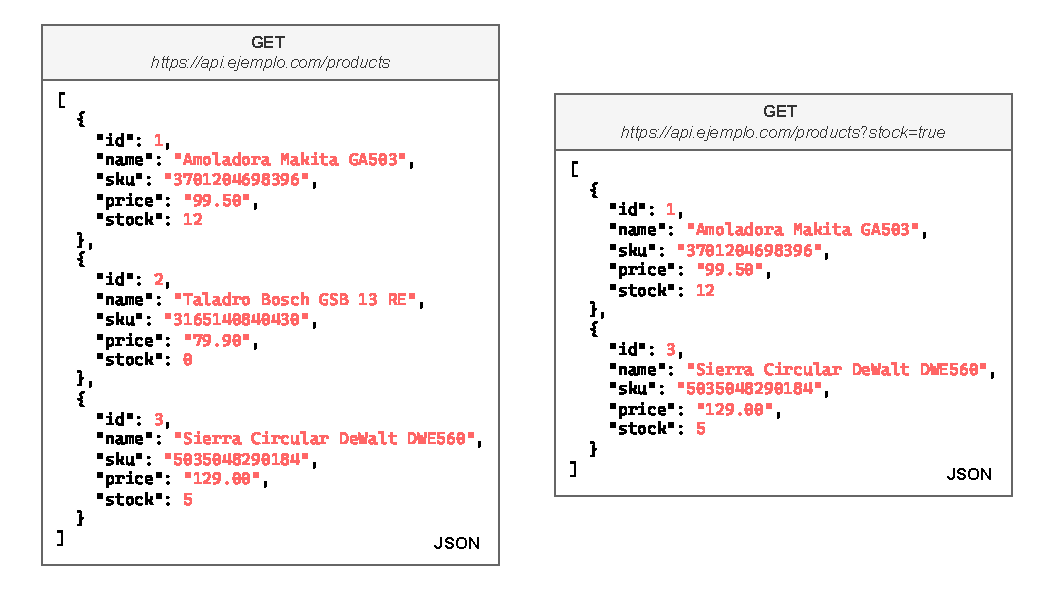
\includegraphics[width=0.8\textwidth]{figures/theoric_frame/query_params_example.pdf}
    \caption{Ejemplo de una respuesta a una petición sin y con \textit{query parameters}.}
    \label{fig:query_params_example}
\end{figure}

% \begin{figure}
%     \centering
%     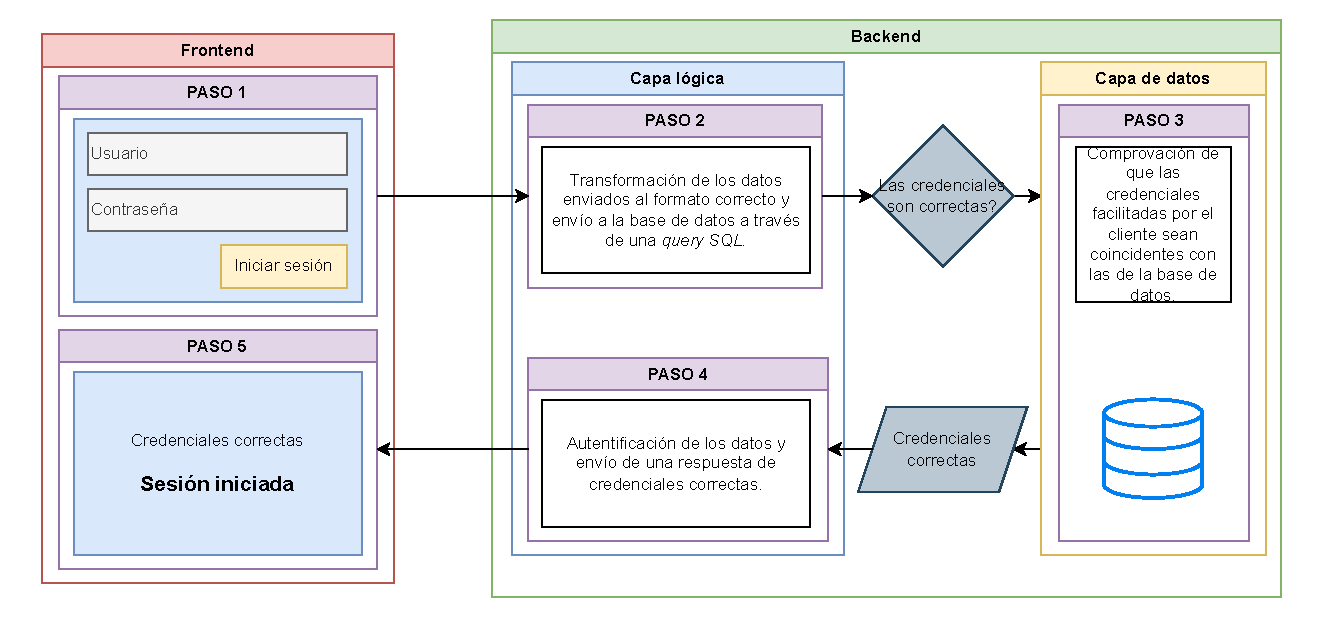
\includegraphics[width=0.8\textwidth]{figures/theoric_frame/use_case.pdf}
%     \caption{Diagrama de flujo del proceso de autenticación de usuario como caso de uso.}
%     \label{fig:use_case}
% \end{figure}

